\section{Gold-PVD}

Als Testsystem für PVD-Prozesse bietet sich mit kristallinem Gold ein System an, dessen Abscheidungsprozess zwar durch Oberflächendiffusion dominiert wird, jedoch kristalline Strukturen bildet und für das ausgiebig erforschte MD-Parametrisierungen existieren.
Da es sich um ein reines Metallsystem handelt, existieren ausreichend getestete EAM-Potentiale, von denen ich mich für die Nutzung der Potentiale aus der Standardbibliothek von LAMMPS\ref{LAMMPS-Ref} entschieden habe.

\subsection{Voruntersuchungen}

Zur Validierung grundlegender Materialeigenschaften wurden Bindungslängen, Dichten und Koordinationszahlen aus einer relaxierten kristallinen Phase untersucht.
Eine Stabilitätsanalyse des Precursormoleküles entfällt, da bei PVD-Prozessen nur einzelne Atome auf die Oberfläche aufgebracht werden.
Zur Bestimmung dieser Werte wurde ein Goldkristall von 40x40x40 \AA Größe auf 1000K aufgeheizt, im kanonischen Ensemble relaxiert und anschließend abgekühlt, wobei bei den entsprechenden Temperaturen die in Tabelle \ref{tab:goldpreresults} gezeigten Werte aufgenommen.
Die Temperaturen ergeben sich aus den Umgebungsbedingungen der Literaturwerte.
Wie man den Ergebnissen ansehen kann, bleibt die Kristallstruktur erwartungsgemäß erhalten (die Schmelztemperatur wurde für die Relaxierung nicht überschritten) und stellt die Literaturwerte in guter Übereinstimmung dar.

\begin{table}[hbtp]
  %% \rowcolors{0}{white}{lightgray} 
  \caption[Eigenschaften von Gold]{Eigenschaften von Gold als Voruntersuchung des PVD-Prozesses. Die Abweichung der Koordinationszahl wird in der Nichtperiodizität der untersuchten Struktur vermutet}
  \label{tab:goldpreresults}
  \begin{tabularx}{\textwidth}{|lXXXX|}
    \hline
    \textbf{unters. Größe} & \textbf{Temperatur} & \textbf{Simulation} & \textbf{Experiment} & \textbf{Abweichung}\\
    \hline
    Bindungslänge & 50 K & 2.885 \AA & 2.884 \AA & 0.05\% \\
    Koordination & 50 K & 12.00 & 12.00 & 0\% \\
    Dichte & 300 K & 18.99 g/cm$^3$ & 19.30 g/cm$^3$ & 1.6\%\\
    Dichte & 500 K & 18.89 g/cm$^3$ & 19.13 g/cm$^3$ & 1.2\%\\
    \hline
  \end{tabularx}
\end{table}

\todo[inline]{Oberflächenvalidierung}

\subsection{Thermische Eigenschaften}

Anders als bei anderen Formulierungen bilden EAM-Potentiale auch thermische Eigenschaften von Metallen ab, die im folgenden kurz für Gold vorgestellt werden.
Dazu wurde die gleiche Teststruktur langsam auf 2000 K, also weit über den Schmelzpunkt von 1337 K, aufgeheizt, während die Materialdichte in Abhängigkeit der Temperatur untersucht wurde.
Die Ergebnisse (Abbildung \ref{fig:goldthermo}) zeigen gute Übereinstimmung mit experimentellen Daten in der Temperaturabhängigkeit der Dichte sowie im Schmelzpunkt.

\begin{figure}[tbp]
  \captionsetup[subfigure]{singlelinecheck=false}
  \def\subfigwidth{0.45\textwidth}
  \begin{subfigure}[t]{\subfigwidth}
    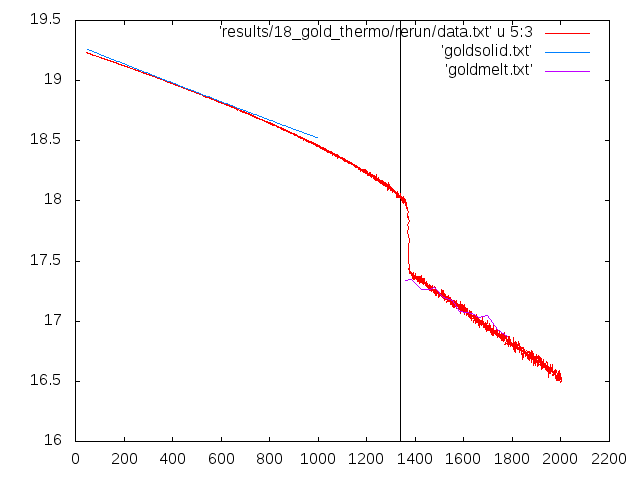
\includegraphics[width=\textwidth]{goldthermo}
    \subcaption{thermische Eigenschaften}
  \end{subfigure}
  \caption[Ergebnisse thermischer Simulationen von Gold]{Ergebnisse thermischer Simulationen von Gold}
  \label{fig:goldthermo}
\end{figure}

\subsection{Prozess-Simulation}

Zur Simulation eines Gold-PVD-Prozesses mit Parsivald wurden die untersuchten Potentialparameter nebst Kristallsubstrat geladen, ein Abscheidungsmodus mit zufälligen Auftreffpositionen in der xy-Ebene gewählt und Relaxationszeiten und Reaktionsnachbarschaftsgrößen gewählt, die in den vorheringen Tests als hinreichend ermittelt wurden.
Damit ergaben sich Reaktionsräume der Größe 37x37x25 \AA mit jeweils ca. 1800 Atomen, Relaxationszeiten von 1.4 ns in 1400 Simulationsschritten und Auftreffgeschwindigkeiten von 4 \AA/ps, die aus üblichen Sputterbedingungen berechnet wurden.\todo{wie berechnet?}

\subsubsection{Strukturierte Substrate}

Als nächste Stufe wurden strukturierte Substrate untersucht, von denen eine Auswahl in Abbildung \ref{fig:goldsubstrate} dargestellt sind.
Diese wurden per Materials Studio präpariert, per Atomsk in ein kompatibles Format überführt und anschließend von Parsivald eingelesen und mit einzelnen Goldatomen beschichtet.

\begin{figure}[bt]
  \captionsetup[subfigure]{singlelinecheck=false}
  \def\subfigwidth{0.31\textwidth}
  \begin{subfigure}[t]{\subfigwidth}
    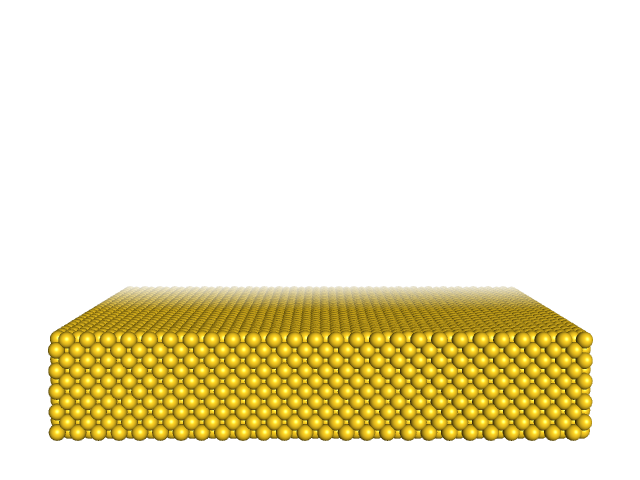
\includegraphics[width=\textwidth]{Au_substrate_flat}
    \subcaption{Flaches Gold-Substrat}
    \label{fig:goldsubstrate-a}
  \end{subfigure}
  \hfill
  \begin{subfigure}[t]{\subfigwidth}
    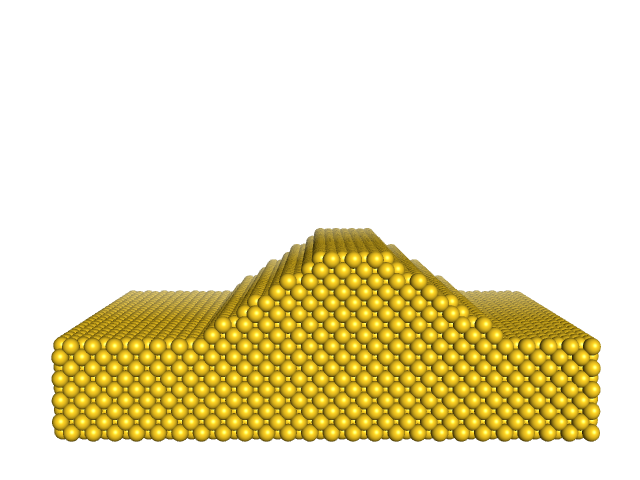
\includegraphics[width=\textwidth]{Au_substrate_step30}
    \subcaption{Gold-Stufe, 30°}
    \label{fig:goldsubstrate-a}
  \end{subfigure}
  \hfill
  \begin{subfigure}[t]{\subfigwidth}
    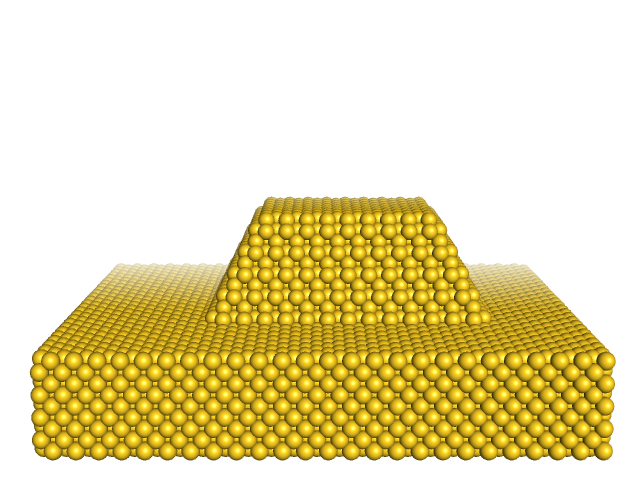
\includegraphics[width=\textwidth]{Au_substrate_tip60}
    \subcaption{Gold-Spitze, 60°}
    \label{fig:goldsubstrate-a}
  \end{subfigure}
  \caption[Strukturierte Goldsubstrate]{Goldsubstrate mit unterschiedlicher Struktur und Breite und Tiefe von 100 \AA.
    Abscheidungen wurden auf flachen Substraten sowie Stufen und Spitzen mit jeweils 15°, 20°, 30°, 45°, 60° und 90° Neigung durchgeführt.}
  \label{fig:goldsubstrate}
\end{figure}

\begin{figure}[bt]
  \captionsetup[subfigure]{singlelinecheck=false}
  \def\subfigwidth{0.31\textwidth}
  \begin{subfigure}[t]{\subfigwidth}
    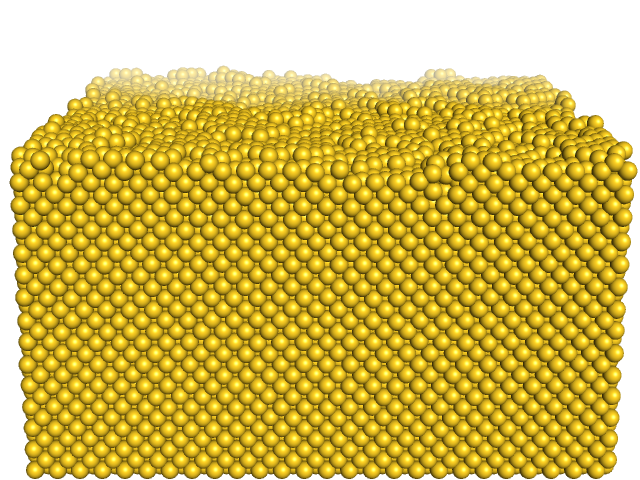
\includegraphics[width=\textwidth]{Au_deposition_flat}
    \subcaption{Abscheidung auf flachem Gold-Substrat}
    \label{fig:goldsubstrate-a}
  \end{subfigure}
  \hfill
  \begin{subfigure}[t]{\subfigwidth}
    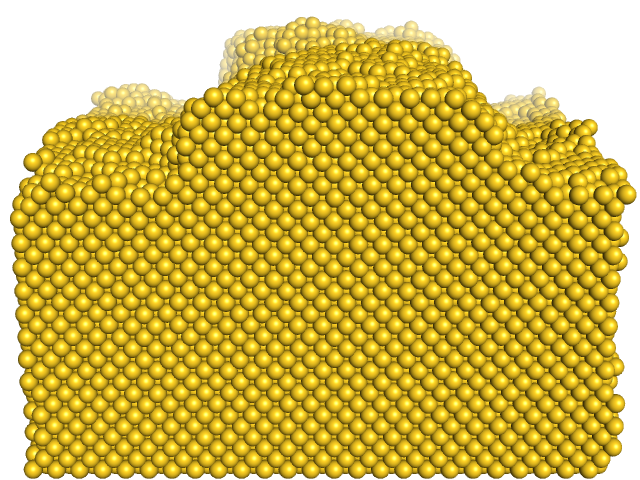
\includegraphics[width=\textwidth]{Au_deposition_step30}
    \subcaption{Abscheidung auf Gold-Stufe, 30°}
    \label{fig:goldsubstrate-a}
  \end{subfigure}
  \hfill
  \begin{subfigure}[t]{\subfigwidth}
    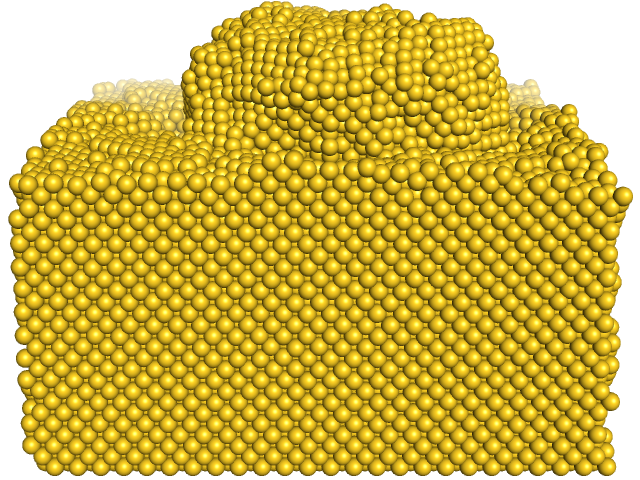
\includegraphics[width=\textwidth]{Au_deposition_tip60}
    \subcaption{Abscheidung auf Gold-Spitze, 60°}
    \label{fig:goldsubstrate-a}
  \end{subfigure}
  \caption[Abscheidung auf strukturierten Substraten]{
    Ergebnis der Abscheidung.
    Die Substratstruktur bleibt erkennbar, wird aber nach oben verstärkt, ansonsten aber kristallin und flach fortgesetzt.
  }
  \label{fig:golddepositions}
\end{figure}

Die Ergebnisse der Gold-Abscheidungen mit Parsivald (Abbildung \ref{fig:golddepositions}) zeigen perfekt fortgesetzte Kristallstrukturen, wobei die Schicht auf dem flachen Substrat nach 10 Kristall-Lagen eine Rauheit von einem Atomdurchmesser zeigt, die weiter beibehalten wird.
Die strukturierten Substrate hingegen zeigen den Trend, die Neigungswinkel an Stufen und Spitzen zu verstärken.
Nach längeren Laufzeiten entstehen somit Überhänge, die durch Abschluss zu Hohlräumen führen, die sich in der Realität durch thermische Relaxation schließen.
Dahinter steht einerseits die Notwendigkeit, Gold-Atome bei Ankunft auf der Oberfläche diffundieren zu lassen, was beim aktuellen Modell nur in Grenzen angewandt wird.

Andererseits steckt dahinter ein methodischer Fehler bei Nutzung von Binning-Methoden:
Die Oberfläche wird aufgrund von Laufzeitbegrenzungen nur entlang der z-Achse bestimmt, woraufhin das neue Atom über einem Atom auf der Oberfläche platziert wird.
Das führt bei Stufen in der Struktur zu Atomen, die immer am oberen Ende einer Kante oder Neigung aufgetragen werden und dort mit statistischer Wahrscheinlichkeit verbleiben.

Eine mögliche Lösung stellt die ausführliche Parametrisierung der Oberfläche dar, beispielsweise per Alpha-Form (Abschnitt \ref{dataalphaform}, über die man die Ereigniswahrscheinlichkeit entsprechend der Einbettungsenergie variierte, angenähert über die Oberflächenkrümmung.
